\documentclass[a4paper,oneside,11pt]{memoir}
\usepackage[utf8]{inputenc} % Input encoding - Depending on editor
\usepackage{lmodern} % Modern LaTeX font
\usepackage[english]{babel} % Language package
\usepackage[T1]{fontenc} % Hyphenation
\usepackage{fix-cm} % Fix for cm
\usepackage{graphicx} % To handle pictures
\usepackage{xcolor} % To define colors
\usepackage{tikz} % Graphical tool
\usepackage{mathtools} % To use \eqref
\usepackage{url} % Use of urls in the text
\usepackage{varioref} % Smarter references
\usepackage{calc}% Auto calculate
\usepackage{lipsum} % Debugging text
\usepackage{sansmath,subfig} % Gives a warning because subfig loads caption

\graphicspath{{figures/}} % Image path

\definecolor{ase_blue}{RGB}{10,55,136}

%---------------------------------------------------------------------------%
%-------------------------- PDF - PROPERTIES -------------------------------%
%---------------------------------------------------------------------------%
% Active links
\usepackage[plainpages=false,pdfpagelabels,pageanchor=false,hidelinks]{hyperref}

\hypersetup{pdfauthor={<The authors>}, pdftitle={<The
    title>},pdfsubject={<The subject>}}

%---------------------------------------------------------------------------%
%---------------------------- Caption Font ---------------------------------%
%---------------------------------------------------------------------------%
\DeclareCaptionFont{sansmath}{\sansmath}
\captionsetup{font={small,sf,sansmath}}
\captionsetup[subfloat]{font={small,sf,sansmath}}

%---------------------------------------------------------------------------%
%---------------------------- MARGIN CONTROL -------------------------------%
%---------------------------------------------------------------------------%
\setlrmarginsandblock{3.5cm}{2.5cm}{*}
\setulmarginsandblock{3cm}{*}{1.2}
\checkandfixthelayout[nearest]
\setlength{\evensidemargin}{\oddsidemargin}

%--------------------------------------------------------------------------%
%------------------------- FRONTPAGE - PROPERTIES -------------------------%
%--------------------------------------------------------------------------%
\usepackage{soul} % Letterspace package
\sodef\an{}{0.05em}{.5em plus.6em}{1em plus.1em minus.1em}
\newcommand\stext[1]{\an{\scshape#1}}
\newcommand{\logoHuge}{\fontsize{0.55cm}{0.8cm}\selectfont}
\newcommand{\SuperHuge}{\fontsize{1.2cm}{1.8cm}\selectfont}

%--------------------------------------------------------------------------%
%------------------------- PAGESTYLE - PROPERTIES -------------------------%
%--------------------------------------------------------------------------%
%\renewcommand{\chaptermark}[1]{\markboth{\MakeUppercase{#1}}{}}

\makepagestyle{ase_report}
\makeoddhead{ase_report}{}{\small\sffamily\leftmark}{}
\makeoddfoot{ase_report}{}{}{\small\sffamily\thepage}

\makeatletter
\makepsmarks{ase_report}{%
  \renewcommand\chaptermark[1]{%
    \markboth{%
      \ifnum \value{secnumdepth} > 1
      \if@mainmatter % 
      \@chapapp\ \thechapter. \ %
      \fi
      \fi
      ##1}{}}%
  \renewcommand\tocmark{\markboth{\contentsname}{\contentsname}}%
  \renewcommand\lofmark{\markboth{\listfigurename}{\listfigurename}}%
  \renewcommand\lotmark{\markboth{\listtablename}{\listtablename}}%
  \renewcommand\bibmark{\markboth{\bibname}{\bibname}}%
  \renewcommand\indexmark{\markboth{\indexname}{\indexname}}%
  \renewcommand\sectionmark[1]{\markright{##1}}%
  \renewcommand\subsectionmark[1]{\markright{##1}}%
  \renewcommand\subsubsectionmark[1]{\markright{##1}}%
}

\copypagestyle{plain}{ase_report}
\makeoddhead{plain}{}{}{}
\makeoddfoot{plain}{}{}{\small\sffamily\thepage}

\pagestyle{ase_report}
\aliaspagestyle{chapter}{plain}

%--------------------------------------------------------------------------%
%--------------------- HEADING - SECTION ----------------------------------%
%--------------------------------------------------------------------------%
\newcommand{\ruledsec}[1]{%
  \Large\bfseries\sffamily\raggedright #1
  \color{ase_blue}\rule[15pt]{\textwidth}{1.0pt}} % Section with ruler
\setsecheadstyle{\ruledsec} % Define section head style

\setfloatlocations{figure}{htp}
\setfloatlocations{table}{htp}

%--------------------------------------------------------------------------%
%--------------------- HEADING - SUBs-SECTION -----------------------------%
%--------------------------------------------------------------------------%
\addtocounter{secnumdepth}{2} % Depth numbering

\setsubsecheadstyle{\large\bfseries\sffamily\raggedright}
\setsubsubsecheadstyle{\Large\bfseries\sffamily\raggedright}

\setsechook{\hangsecnum} % Hang the section number in margin
\setsubsechook{\defaultsecnum} % Don't do this on the subsections
\setsubsubsechook{\defaultsecnum}
\setaftersecskip{5pt} % Default skip between the section and text

%--------------------------------------------------------------------------%
%------------------------- TOC - PROPERTIES -------------------------------%
%--------------------------------------------------------------------------%
\raggedbottomsectiontrue % The page may not be strected on page breaks
\setsecnumdepth{subsubsection} % Set section depth in the TOC
\maxsecnumdepth{subsubsection} % Max of section depth in the TOC
\settocdepth{subsection} % Up to and including subsection

\setlength{\cftbeforechapterskip}{1.0em plus 0.1em minus 0.1em} % Space from chapters
%\chapterprecistoc{Text in TOC}

\addto\captionsenglish{
  \renewcommand*{\cftchaptername}{Chapter{\space}}
  \renewcommand*{\cftfigurename}{Fig.{\space}}
  \renewcommand*{\contentsname}{Table of Contents}
  \renewcommand*{\abstractname}{Abstract}
  \renewcommand*{\listfigurename}{List{\space}of{\space}Figures}
  \renewcommand*{\listtablename}{List{\space}of{\space}Tables}
  \renewcommand*{\appendixtocname}{Appendices}
  \renewcommand*{\appendixpagename}{Appendices}
}

\addto\captionsdanish{
  \renewcommand*{\cftchaptername}{Kapitel\space}
  \renewcommand*{\cftfigurename}{Fig.\space}
  \renewcommand*{\abstractname}{Resumé}
  \renewcommand*{\contentsname}{Indholdsfortegnelse}
  \renewcommand*{\listfigurename}{Liste{\space}af{\space}Figurer}
  \renewcommand*{\listtablename}{Liste{\space}af{\space}Tabeller}
  \renewcommand*{\appendixtocname}{Appendikser}
  \renewcommand*{\appendixpagename}{Appendikser}
}
%--------------------------------------------------------------------------%
%------------------------- CHAPTER STYLE ----------------------------------%
%--------------------------------------------------------------------------%
\makechapterstyle{ase_chapterstyle}{
  \setlength{\beforechapskip}{30pt}
  \setlength{\afterchapskip}{1.5cm}
  \renewcommand*{\printchaptername}{}
  \renewcommand*{\chapnumfont}{\normalfont\sffamily\bfseries\fontsize{60}{0}\selectfont}
  \renewcommand*{\printchapternum}{
    \flushright
    \begin{tikzpicture}
      \draw[fill,color=ase_blue] (0,0) rectangle (2cm,2cm);
      \draw[color=white] (1cm,1cm) node { \chapnumfont\thechapter };
    \end{tikzpicture}
  }
  \renewcommand*{\chaptitlefont}{\normalfont\sffamily\Huge\bfseries\color{black}}
  \renewcommand*{\printchaptertitle}[1]{%
    \raggedright\chaptitlefont\parbox[t]{\textwidth}{\raggedright##1}}
}

\chapterstyle{ase_chapterstyle}

%--------------------------------------------------------------------------%
%------------------------- USER DEFINED COMMANDS --------------------------%
%--------------------------------------------------------------------------%
% Define some macros


\begin{document}
%\includeonly{testing} %If you don't want to compile every time
%--------------------------------------------------------------------------%
%------------------------- FRONT MATTER -----------------------------------%
%--------------------------------------------------------------------------%
\frontmatter
% Frontpage - Titlingpage from Memoir class 
\begin{titlingpage}
  
  \thispagestyle{empty}
  
  % Define the colourbar on the frontpage
  \begin{tikzpicture}[remember picture,overlay]
    \coordinate [below=2.5cm] (midpoint) at (current page.north);

    \node [name=colourbar,
    anchor=base,
    fill=ase_blue,
    text = white,
    minimum width=\paperwidth,
    minimum height=1cm] at (midpoint) {\logoHuge{\textsc{{Aarhus School Of
            Engineering}}}};

    % Define the point where the logo will go
    \coordinate [right=4cm] (ase_logo) at (colourbar.west);

    % Set coordinate system origin
    \begin{scope}[shift=(ase_logo)]
      % Draw the outline
      \filldraw [white] (1.2,0.85) -- (-1.6,0.85) -- (-2.3,-0.85) -- (1.2,-0.85) --cycle;
      % Include the logo
      \node [xshift=-0.5cm]{\includegraphics[width=3cm]{ase_logo.png}};
    \end{scope}
  \end{tikzpicture}

  % Temporary center margins
  \begin{adjustwidth}{-0.5cm}{0cm}
    \vspace*{\stretch{0.5}}
    \centering
    { \setlength{\baselineskip}{32pt}
      {\SuperHuge \stext{Fast Video Stabilization for Hand-held Devices} 
      }\par
      \stext{<Subtitle Example : Implemented on a Andriod system>}
      \par\vspace*{4\onelineskip}
      \par
      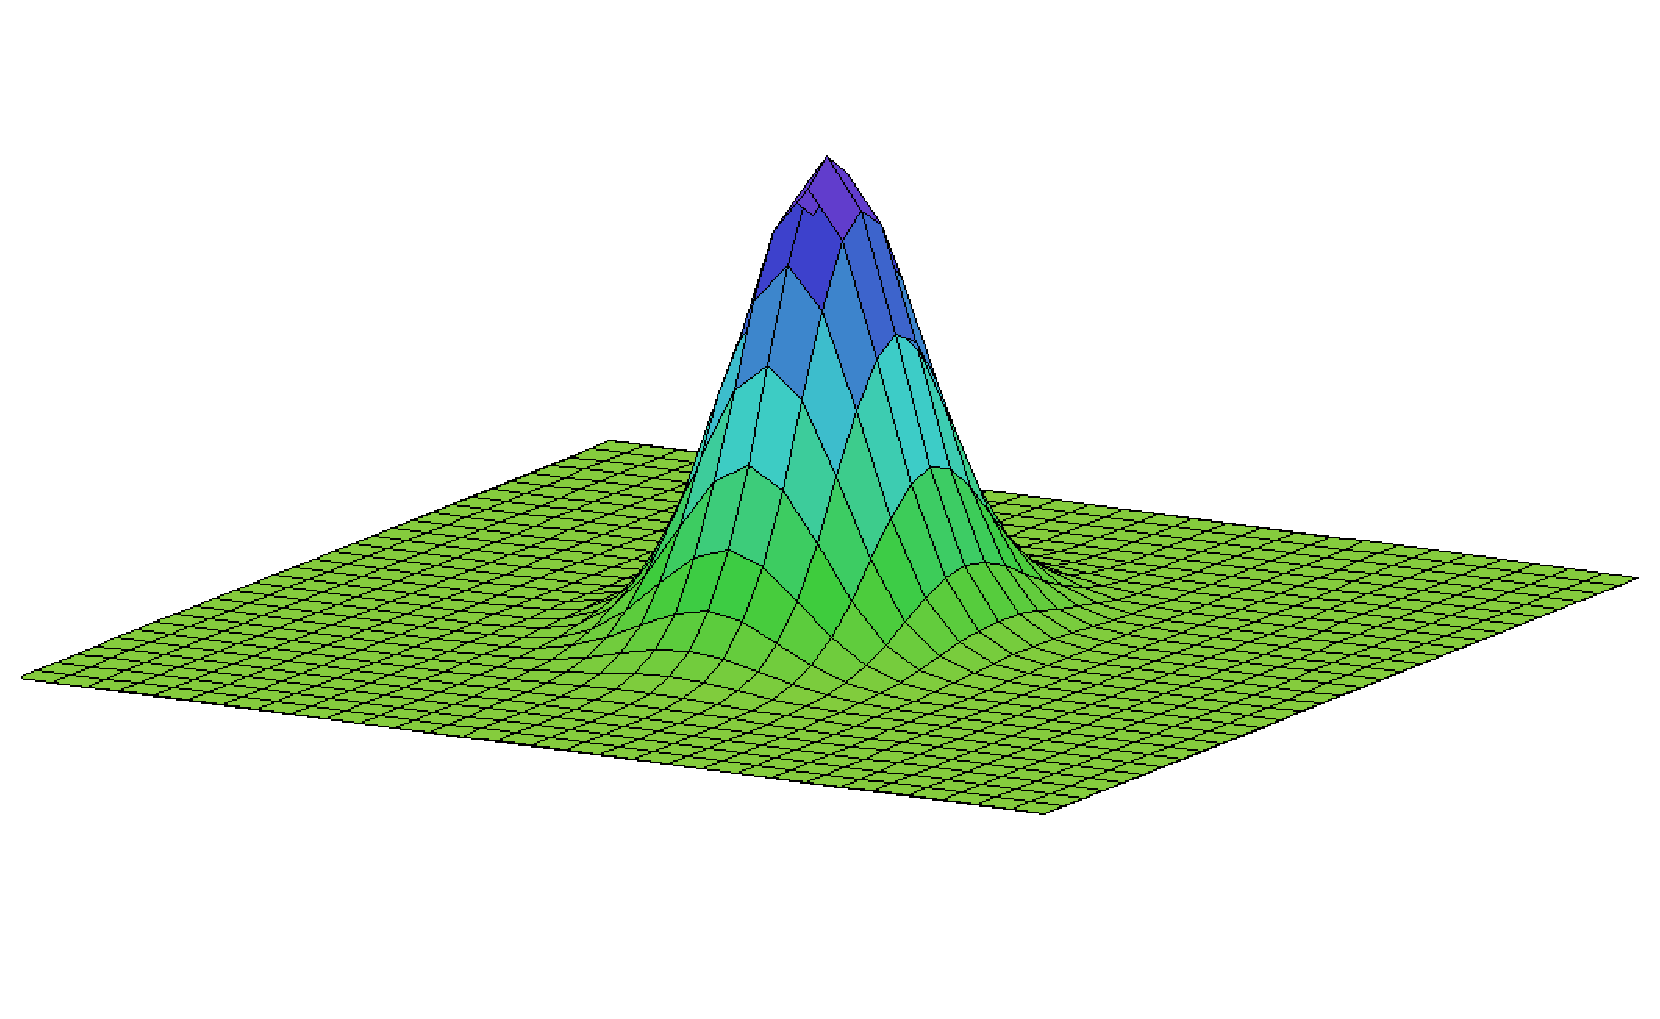
\includegraphics[width=10cm]{frontpage}
      \par\vspace*{4\onelineskip}
      \textbf{\stext{Engineering Research and Development Project}}\par
      \par\vspace*{2\onelineskip}
      % Make a table to make the --- align
      \begin{center}
        \begin{tabular}{lcl}
          \large\stext{Anders And Andersen} & \large\stext{---} &
          \large\stext{20100000} \\ [1ex]
          % To use danish letters with the UTF8 and soul package
          % we type \o = ø , \ae = æ, \aa = å, \AA = Å, etc.
          \large\stext{S\o ren S\o rensen} & \large\stext{---} & 
          \large\stext{20100001} \\ [1ex]
        \end{tabular}
      \end{center}
    }
    \vfill
    \stext{Supervisor: Henrik Karstoft}\hfill
    \stext{21. januar 2011}

    \enlargethispage{3.5\onelineskip}
  \end{adjustwidth}
\end{titlingpage}







 % Include the frontpage

% Page number in roman style
\pagenumbering{roman}
\addcontentsline{toc}{chapter}{\abstractname}
\thispagestyle{plain}
\newcommand{\newresumemeargin}{3.5cm}
\newcommand{\resumeheadingsize}{\Large}
\newgeometry{left=\newresumemeargin, right=\newresumemeargin}

% Kort oversigt over den faglige gennemgang og konklusionen (senedenfor). Det bør indledes med en meget kort redegørelse for emnet, afgrænsningen og synsvinklen. Formålet er kun at fortælle læseren, hvad han kan bruge denne rapport til.

\centerline{\resumeheadingsize\bf Resumé}
\vskip 0.3cm
\lipsum[2-3]
\vskip 4em

\centerline{\resumeheadingsize\bf Abstract}
\vskip 0.3cm
\lipsum[2-3]

\restoregeometry
\clearpage

\addcontentsline{toc}{chapter}{\contentsname}
\thispagestyle{empty}
\tableofcontents*

\clearpage

\addcontentsline{toc}{chapter}{\listfigurename}
\thispagestyle{empty}
\listoffigures*
\clearpage

\addcontentsline{toc}{chapter}{\listtablename}
\thispagestyle{empty}
\listoftables*

%--------------------------------------------------------------------------%
%------------------------- MAIN MATTER ------------------------------------%
%--------------------------------------------------------------------------%
\mainmatter
\chapter{Introduction of the ASE Template}
\label{chap:f}
\lipsum[1]

\begin{figure}[htp]
  \centering
  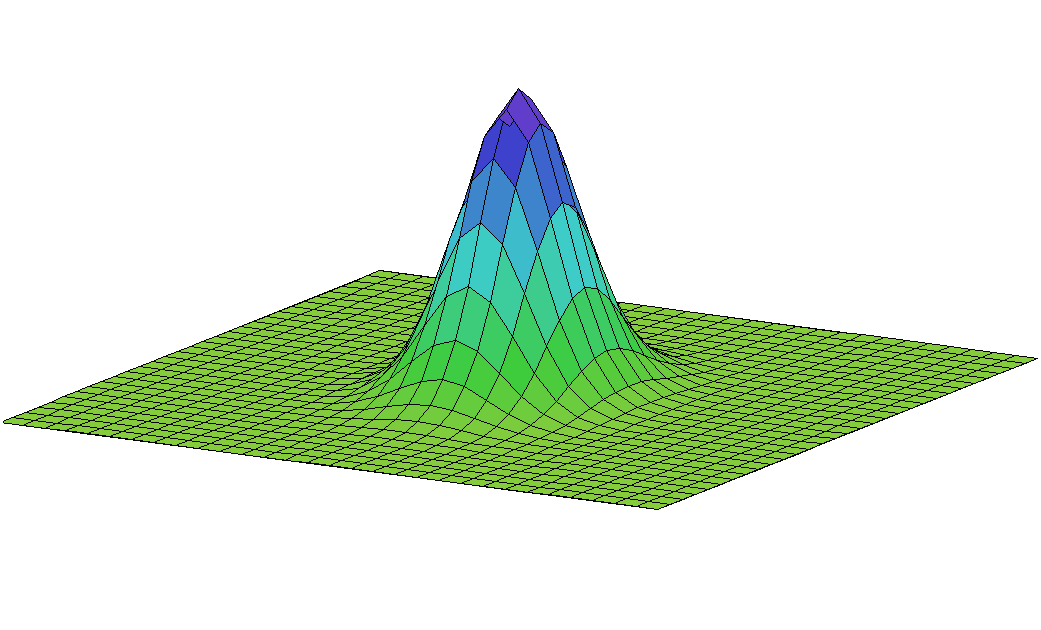
\includegraphics[width=6cm]{frontpage.png}
  \caption{Test of a picture}
  \label{fig:test}
\end{figure}

\lipsum[1]
\begin{figure}[ht]
  \begin{minipage}[htp]{0.48\linewidth}
    \centering
    \includegraphics[draft,width=\linewidth]{ase_logo.png}
  \end{minipage}
  \hfill
  \begin{minipage}[htp]{0.48\linewidth}
    \centering
      \includegraphics[draft,width=\linewidth]{ase_logo.png}
  \end{minipage}
    \caption{Pictures side by side}
  \label{fig:test1}
\end{figure}

\lipsum[1]

\section{Section dummy text}

\lipsum[1]

\[
 \frac{n!}{k!(n-k)!} = \binom{n}{k}
\]
\begin{equation}
  \frac{n!}{k!(n-k)!} = \binom{n}{k}
\end{equation}
\lipsum[1]

\subsection{Subsection dummy text}

\lipsum[1]

\begin{figure}
    \subfloat[Subcaption $1+a$]{\framebox[7cm]{First}} \hfill
    \subfloat[Subcaption $1+b$]{\framebox[7cm]{Second}}
    \caption{Main caption $1+x$} 
\end{figure}

\lipsum[1]
\section{Another dummy section}

\lipsum

Test of the reference system \cite{Rabiner89}. % Include the chapters

Test of the reference system \cite{Rabiner89}.
%--------------------------------------------------------------------------%
%------------------------- BACK MATTER ------------------------------------%
%--------------------------------------------------------------------------%

\appendixpage

\appendix
%\addtocontents{toc}{\cftpagenumbersoff{chapter}}
\chapter{A random appendix}
\label{appendixA}

\lipsum[1-5]

\backmatter

%\bibliographystyle{plain} % eller en anden stil
\bibliographystyle{ieeetr}
\bibliography{reference/my-bibliography-file}

\end{document}

%%% Local Variables: 
%%% mode: latex
%%% TeX-master: t
%%% End: 